% !TeX spellcheck = ru_RU
% !TEX root = vkr.tex

\section{Эксперимент}

\subsection{Условия эксперимента}

Экспериментальное исследование проводилось на трёх аппаратных платформах: двух одноплатных компьютерах на базе архитектуры RISC-V (Banana Pi BPI-F3 и StarFive VisionFive 2) и одной референсной платформе на базе архитектуры x86-64 со встроенной графикой Intel (Intel Core i9-12900H с Intel Iris Xe Graphics).

Характеристики платформ подробно описаны в разделе~2.4. Кратко:
\begin{itemize}
    \item \textbf{Banana Pi BPI-F3}: SpacemiT K1 (8 ядер RISC-V @ 2.0 ГГц), IMG BXE-2-32 GPU, 16 ГБ LPDDR4-2666;
    \item \textbf{StarFive VisionFive 2}: JH7110 (4 ядра RISC-V @ 1.5 ГГц), IMG BXE-4-32 MC1 GPU, 8 ГБ LPDDR4-2800;
    \item \textbf{Intel Iris Xe}: Intel Core i9-12900H (14 ядер @ до 5.0 ГГц), Intel Iris Xe Graphics (96 EU), 24 ГБ DDR5-4800.
\end{itemize}

Для каждой конфигурации параметров и каждого ядра выполнялось по 100 прогонов операции умножения матриц. Измерялось только время выполнения OpenCL ядра, без учёта времени на подготовку данных, их копирование в память устройства и обратно. Это позволило получить чистую оценку вычислительной производительности различных реализаций алгоритма. Для обработки результатов использовалось среднее арифметическое значение времени выполнения.

Для обеспечения стабильности измерений на RISC-V платформах использовалось пассивное охлаждение, частоты процессоров работали в штатном режиме с динамическим управлением. Скрипты для автоматизации тестирования и обработки результатов доступны в форке репозитория MyGEMM~\cite{mygemm_repo_test}.

\subsection{Тестовые данные}

В качестве тестовых данных использовались квадратные матрицы размером $1024 \times 1024$ элементов типа \texttt{float} (32-бит). Размер матриц был выбран достаточно большим для выявления различий в производительности различных оптимизаций, но при этом умещающимся в память всех тестируемых устройств.

Тестировались 11 ядер библиотеки MyGEMM (от наивной реализации до продвинутых оптимизаций) с различными наборами параметров конфигурации. Для ядер 1--3 варьировался параметр TS (Tile Size) со значениями из множества \{8, 16\}. Значение TS=32 не тестировалось, поскольку оно приводит к созданию рабочей группы размером $32 \times 32 = 1024$ потока, что превышает аппаратное ограничение в 32 потока на RISC-V платформах. Попытки запуска с TS=32 приводили к ошибке выполнения ``Invalid work group size''.

Для ядер 4--10 тестировались комбинации параметров TSM и TSN из множества \{32, 64, 128\} с соответствующими значениями WPTM и WPTN, что дало 9 уникальных конфигураций для каждого ядра. Ядро 11 имеет фиксированную конфигурацию параметров, определённую реализацией clBLAS.

Все конфигурации параметров были подобраны с учётом ограничения максимального размера рабочей группы в 32 потока на RISC-V платформах.

\subsection{Результаты измерений}

Результаты экспериментов представлены на рисунках~\ref{fig:perf_bananapi}--\ref{fig:perf_intelxe} для каждой из тестируемых платформ. На графиках показано среднее время выполнения операции умножения матриц в секундах для различных ядер и конфигураций параметров.

\begin{figure}[ht]
\centering
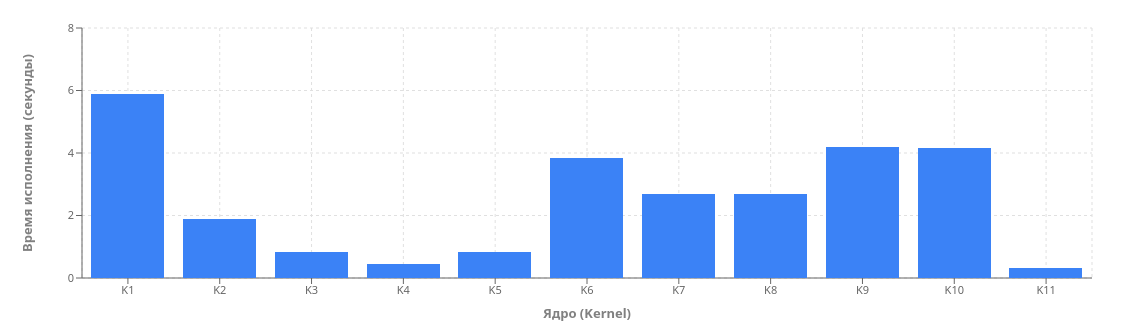
\includegraphics[width=0.95\textwidth]{figures/banana_pi_83232.png}
\caption{Производительность ядер MyGEMM на платформе Banana Pi BPI-F3 для конфигурации TS=8, TSM=32, TSN=32}
\label{fig:perf_bananapi}
\end{figure}

\begin{figure}[ht]
\centering
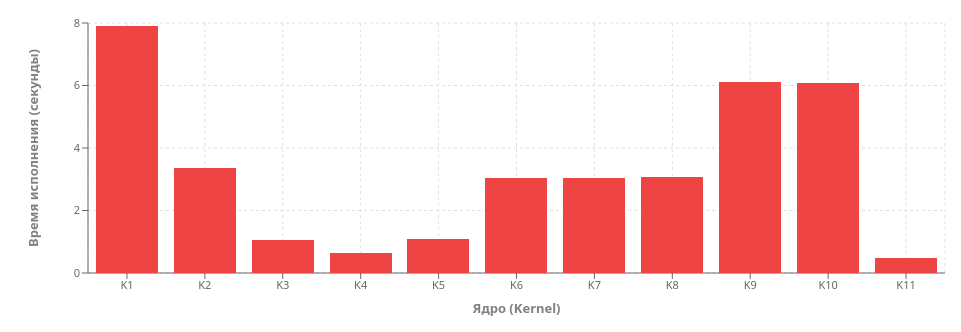
\includegraphics[width=0.95\textwidth]{figures/starfive_83232.png}
\caption{Производительность ядер MyGEMM на платформе StarFive VisionFive 2 для конфигурации TS=8, TSM=32, TSN=32}
\label{fig:perf_starfive}
\end{figure}

\begin{figure}[ht]
\centering
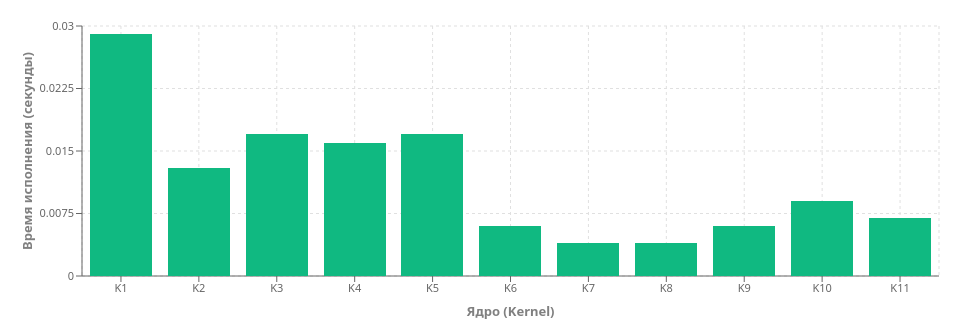
\includegraphics[width=0.95\textwidth]{figures/intel_xe_83232.png}
\caption{Производительность ядер MyGEMM на референсной платформе Intel Iris Xe для конфигурации TS=8, TSM=32, TSN=32}
\label{fig:perf_intelxe}
\end{figure}

\subsubsection{Анализ результатов}

Экспериментальные данные демонстрируют значительные различия в производительности между RISC-V платформами и референсной системой Intel Xe. Референсная платформа Intel Xe показывает время выполнения в диапазоне 0.004--0.029 секунд для различных ядер, что в среднем в 200--400 раз быстрее, чем RISC-V платформы.

Среди RISC-V платформ Banana Pi BPI-F3 демонстрирует лучшую производительность по сравнению со StarFive VisionFive 2, что объясняется более высокой тактовой частотой (2.0 ГГц против 1.5 ГГц) и большим количеством вычислительных ядер (8 против 4). Среднее время выполнения на Banana Pi составляет 0.3--11 секунд, на StarFive -- 0.5--9 секунд.

Ключевые наблюдения:
\begin{itemize}
    \item \textbf{Наилучший результат}: Ядро 11 (clBLAS-подход) демонстрирует наилучшую производительность на всех трёх платформах. На Banana Pi время выполнения составляет 0.32 сек, на StarFive -- 0.49 сек, на Intel Xe -- 0.007 сек. Это ядро не использует локальную память и полностью полагается на регистровую блокировку с векторными типами данных.
    
    \item \textbf{Проблемы векторизации}: Ядра 6--10, активно использующие векторизацию загрузки/записи данных, показывают неожиданно низкую производительность на RISC-V платформах. Время выполнения достигает 9--11 секунд, что в 10--30 раз медленнее более простых ядер 3--5. Это указывает на недостаточную оптимизацию драйверов OpenCL для векторных операций на архитектуре RISC-V.
    
    \item \textbf{Эффективность базовых оптимизаций}: Ядра 2--5, использующие блочную обработку с локальной памятью и work-per-thread оптимизацию, показывают хороший результат. Ядра 4 и 5 (2D регистровая блокировка с транспонированием) достигают времени 0.3--0.6 секунд на RISC-V, что в 10--25 раз быстрее наивной реализации (ядро 1).
    
    \item \textbf{Ограничения архитектуры}: Жёсткое ограничение размера рабочей группы в 32 потока на RISC-V платформах существенно ограничивает возможности оптимизации. Многие конфигурации параметров, эффективные на дискретных GPU, не могут быть использованы на RISC-V.
\end{itemize}

Полученные результаты показывают, что для достижения приемлемой производительности на RISC-V платформах следует отдавать предпочтение подходу, реализованному в ядре 11 (clBLAS), который не использует локальную память и основывается на регистровой блокировке. Ядра с активной векторизацией (6--10) следует избегать до улучшения драйверов OpenCL.